\documentclass{article}
\usepackage[utf8]{inputenc}
\usepackage[margin=1in]{geometry}
\usepackage{listings}
\usepackage{xcolor}
\usepackage{booktabs}
\usepackage{graphicx}

\definecolor{codegreen}{rgb}{0,0.6,0}
\definecolor{codegray}{rgb}{0.5,0.5,0.5}
\definecolor{codepurple}{rgb}{0.58,0,0.82}
\definecolor{backcolour}{rgb}{0.95,0.95,0.92}

\lstdefinestyle{mystyle}
{
	backgroundcolor=\color{backcolour},   
	commentstyle=\color{codegreen},
	keywordstyle=\color{magenta},
	numberstyle=\tiny\color{codegray},
	stringstyle=\color{codepurple},
	basicstyle=\ttfamily\footnotesize,
	breakatwhitespace=false,         
	breaklines=true,                 
	captionpos=b,                    
	keepspaces=true,                 
	numbers=left,                    
	numbersep=5pt,                  
	showspaces=false,                
	showstringspaces=false,
	showtabs=false,                  
	tabsize=2
}

\lstset{style=mystyle}
\begin{document}
\begin{titlepage} % Suppresses displaying the page number on the title page and the subsequent page counts as page 1
		
		\raggedleft\rule{1pt}{\textheight} % Vertical line
		\hspace{0.05\textwidth} % Whitespace between the vertical line and title page text
		\parbox[b]{0.75\textwidth}
		{ % Paragraph box for holding the title page text, adjust the width to move the title page left or right on the page
			
			{\Huge\bfseries MIT World Peace University \\[0.5\baselineskip] \ Data Base Management System}\\[2\baselineskip] % Title
			{\large\textit{Assignment 3}}\\[4\baselineskip] % Subtitle or further description
			{\Large\textsc{Naman Soni Roll No. 10\\
			Sayyam Saboo Roll No. 30}} % Author name, lower case for consistent small caps
			
			\vspace{0.5\textheight} % Whitespace between the title block and the publisher
		}
		
\end{titlepage}
\tableofcontents
\pagebreak

\section{\textbf{Introduction}}
Hospital management system is a digital platform that enables hospitals to manage their administrative and clinical workflows efficiently. The aim of this project is to design and develop a hospital management system using the Python programming language and MySql.

\section{\textbf{Problem Statement}}
Traditional hospital management systems are often inefficient and time-consuming, leading to delays and errors in patient care. The hospital management system aims to solve these problems by digitizing administrative and clinical workflows, providing real-time access to patient information, and automating processes.

\section{\textbf{Objective}}
The objectives of the project are:
\begin{itemize}
    \item To create a digital platform for managing administrative and clinical workflows in hospitals.
    \item To provide real-time access to patient information to hospital staff.
    \item To automate processes to reduce delays and errors in patient care.
    \item To ensure data security and privacy.
    
\end{itemize}

\section{\textbf{System Implementation}}
The hospital management system is implemented using the Python programming language. The following technologies are used in the implementation:
\begin{itemize}
    \item MySQL\: This is a database management system that is used to store the hospital data.
    The implementation details include creating the database schema, creating the Django models, views, and templates, and integrating the system with the database.
    
\end{itemize}


\section{\textbf{Normalization}}
The table in the project is in 1NF.

\section{\textbf{ER Diagram}}
\begin{center}
    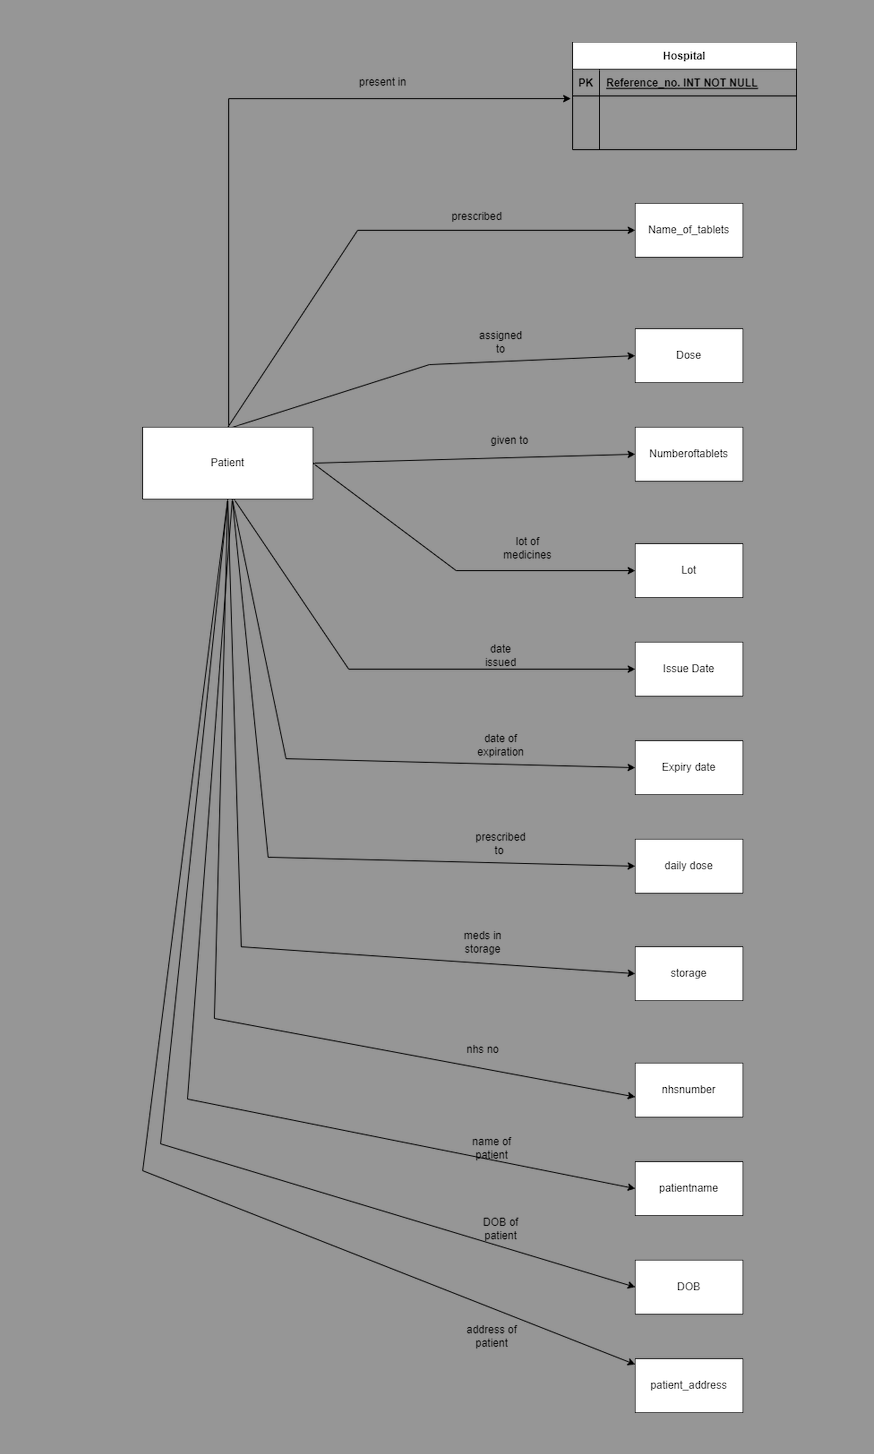
\includegraphics[scale = 0.8]{ERDiagram.png}
\end{center}

\section{\textbf{User Interface}}
\begin{center}
    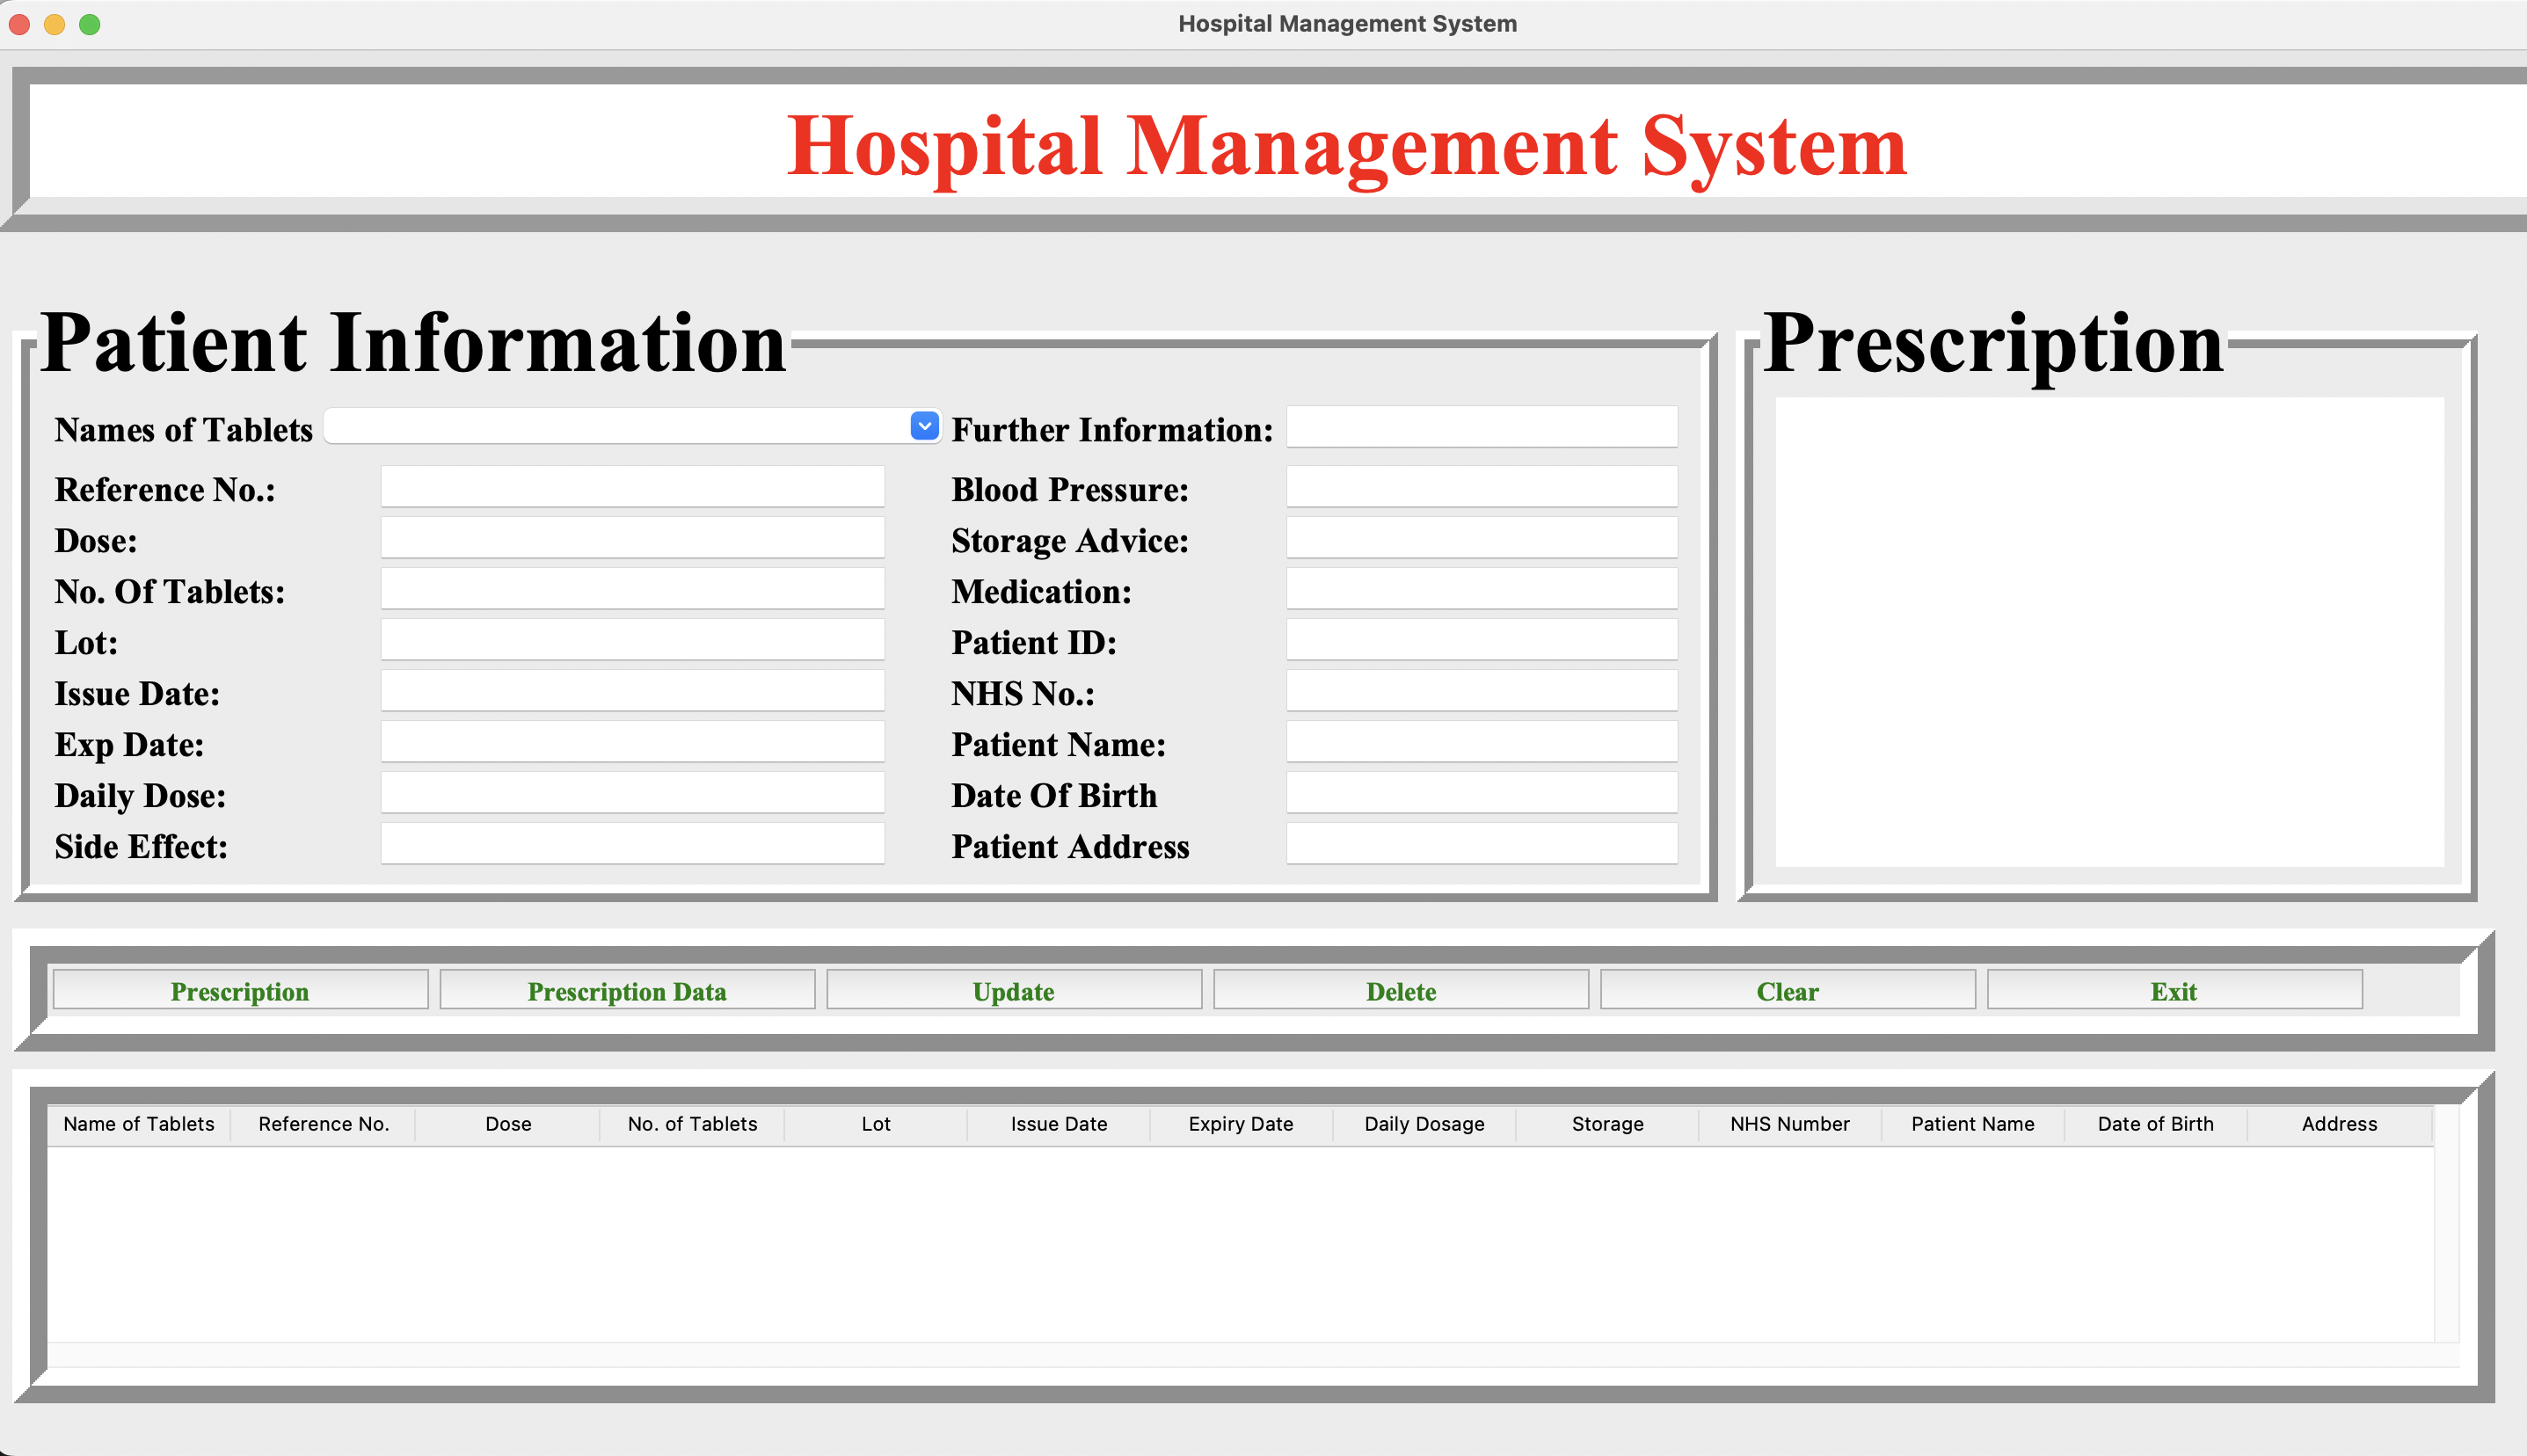
\includegraphics[scale = 0.35]{UI.png}
\end{center}

\section{\textbf{Code}}
\begin{lstlisting}[language=Python, caption=Hospital Management.py]
	from tkinter import *
	from tkinter import ttk
	import random
	import time
	import datetime
	from tkinter import messagebox
	import mysql.connector
	
	
	class Hospital:
		def __init__(self, root):
			self.root = root
			self.root.title("Hospital Management System")
			self.root.geometry("1280x720+0+0")
			self.conn = mysql.connector.connect(host="127.0.0.1", username="root", password="Sayyam@123", database="mydata")
			self.my_cursor = self.conn.cursor()
			self.Nameoftablets = StringVar()
			self.ref = StringVar()
			self.Dose = StringVar()
			self.NoofTablets = StringVar()
			self.Lot = StringVar()
			self.Issuedate = StringVar()
			self.Expdate = StringVar()
			self.DailyDose = StringVar()
			self.sideEffect = StringVar()
			self.FurtherInformation = StringVar()
			self.BloodP = StringVar()
			self.StorageAdvice = StringVar()
			self.DrivingUsingMachine = StringVar()
			self.HowtoUseMedications = StringVar()
			self.PatientId = StringVar()
			self.nhsNumber = StringVar()
			self.PatientName = StringVar()
			self.DateOfBirth = StringVar()
			self.PatientAddress = StringVar()
			
	
			lbltitle = Label(self.root, bd=20, relief=RIDGE, text="Hospital Management System",fg="red", bg="white", font=("Times New Roman", 40, "bold"))
			lbltitle.pack(side=TOP, fill=X)
	
			# =========================DataFrame========================
			Dataframe = Frame(self.root, bd=20, relief=RIDGE)
			Dataframe.place(x=0, y=110, width=1280, height=348)
	
	
			dataframeLeft = LabelFrame(Dataframe, bd=8, relief=RIDGE, padx=8,
									   font=("arial", 11, "bold"), text="Patient Information")
			dataframeLeft.place(x=10, y=3, width=850, height=300)
	
			dataframeRight = LabelFrame(Dataframe, bd=8, relief=RIDGE, padx=8,
										font=("arial", 11, "bold"), text="Prescription")
			dataframeRight.place(x=865, y=3, width=350, height=300)
	
			# =========================Buttons Frame========================
	
	
			ButtonFrame = Frame(self.root, bd=16, relief=RIDGE)
			ButtonFrame.place(x=0, y=460, width=1280, height=58)
	
	
			# =========================Details Frame========================
	
			DetailsFrame = Frame(self.root, bd=16, relief=RIDGE)
			DetailsFrame.place(x=0, y=520, width=1280, height=165)
	
		# =========================dataframeLeft========================
	
			lblNameTablet = Label(dataframeLeft, text="Names of Tablets",
								  font=("arial", 11, "bold"), padx=1, pady=4)
			lblNameTablet.grid(row=0, column=0)
	
			comNameTablet = ttk.Combobox(dataframeLeft, textvariable=self.Nameoftablets, state="readonly",
										 font=("arial", 11, "bold"),
										 width=33)
			comNameTablet["values"] = (
				"Dolo 350", "Paracetamol", "Aspirin", "Crocin", "Monter LC", "Neprocin")
			comNameTablet.grid(row=0, column=1)
	
			lblref = Label(dataframeLeft, font=("arial", 11, "bold"),
						   text="Reference No.:", padx=1)
			lblref.grid(row=1, column=0, sticky=W)
			textref = Entry(dataframeLeft, font=(
				"arial", 11, "bold"), textvariable=self.ref, width=33)
			textref.grid(row=1, column=1)
	
			lbldose = Label(dataframeLeft, font=("arial", 11, "bold"),
							text="Dose:", padx=1)
			lbldose.grid(row=2, column=0, sticky=W)
			textdose = Entry(dataframeLeft, font=(
				"arial", 11, "bold"), textvariable=self.Dose, width=33)
			textdose.grid(row=2, column=1)
	
			lblNoOfTablets = Label(dataframeLeft, font=("arial", 11, "bold"),
								   text="No. Of Tablets:", padx=1)
			lblNoOfTablets.grid(row=3, column=0, sticky=W)
			textNoOfTablets = Entry(dataframeLeft, font=(
				"arial", 11, "bold"), textvariable=self.NoofTablets, width=33)
			textNoOfTablets.grid(row=3, column=1)
	
			lblLot = Label(dataframeLeft, font=("arial", 11, "bold"),
						   text="Lot:", padx=1)
			lblLot.grid(row=4, column=0, sticky=W)
			textLot = Entry(dataframeLeft, font=(
				"arial", 11, "bold"), textvariable=self.Lot, width=33)
			textLot.grid(row=4, column=1)
	
			lblissuedate = Label(dataframeLeft, font=("arial", 11, "bold"),
								 text="Issue Date:", padx=1)
			lblissuedate.grid(row=5, column=0, sticky=W)
			textissuedate = Entry(dataframeLeft, font=(
				"arial", 11, "bold"), textvariable=self.Issuedate, width=33)
			textissuedate.grid(row=5, column=1)
	
			lblexpirydate = Label(dataframeLeft, font=("arial", 11, "bold"),
								  text="Exp Date:", padx=1)
			lblexpirydate.grid(row=6, column=0, sticky=W)
			textexpirydate = Entry(dataframeLeft, font=(
				"arial", 11, "bold"), textvariable=self.Expdate, width=33)
			textexpirydate.grid(row=6, column=1)
	
			lbldailydose = Label(dataframeLeft, font=("arial", 11, "bold"),
								 text="Daily Dose:", padx=1)
			lbldailydose.grid(row=7, column=0, sticky=W)
			textdailydose = Entry(dataframeLeft, font=(
				"arial", 11, "bold"), textvariable=self.DailyDose, width=33)
			textdailydose.grid(row=7, column=1)
	
			lblsideeffect = Label(dataframeLeft, font=("arial", 11, "bold"),
								  text="Side Effect:", padx=1)
			lblsideeffect.grid(row=8, column=0, sticky=W)
			textsideeffect = Entry(dataframeLeft, font=(
				"arial", 11, "bold"), textvariable=self.sideEffect, width=33)
			textsideeffect.grid(row=8, column=1)
	
			lblfurtherinfo = Label(dataframeLeft, font=("arial", 11, "bold"),
								   text="Further Information:", padx=1)
			lblfurtherinfo.grid(row=0, column=3, sticky=W)
			textfurtherinfo = Entry(dataframeLeft, font=(
				"arial", 11, "bold"), textvariable=self.FurtherInformation, width=25)
			textfurtherinfo.grid(row=0, column=4)
	
			lblbloodp = Label(dataframeLeft, font=("arial", 11, "bold"),
							  text="Blood Pressure:", padx=1)
			lblbloodp.grid(row=1, column=3, sticky=W)
			textbloodp = Entry(dataframeLeft, font=(
				"arial", 11, "bold"), textvariable=self.BloodP, width=25)
			textbloodp.grid(row=1, column=4)
	
			lblstorageadvice = Label(dataframeLeft, font=("arial", 11, "bold"),
									 text="Storage Advice:", padx=1)
			lblstorageadvice.grid(row=2, column=3, sticky=W)
			textstorageadvice = Entry(dataframeLeft, font=(
				"arial", 11, "bold"), textvariable=self.StorageAdvice, width=25)
			textstorageadvice.grid(row=2, column=4)
	
			lblmedication = Label(dataframeLeft, font=("arial", 11, "bold"),
								  text="Medication:", padx=1)
			lblmedication.grid(row=3, column=3, sticky=W)
			textmedication = Entry(dataframeLeft, font=(
				"arial", 11, "bold"), textvariable=self.HowtoUseMedications, width=25)
			textmedication.grid(row=3, column=4)
	
			lblpatientid = Label(dataframeLeft, font=("arial", 11, "bold"),
								 text="Patient ID:", padx=1)
			lblpatientid.grid(row=4, column=3, sticky=W)
			textpatientid = Entry(dataframeLeft, font=(
				"arial", 11, "bold"), textvariable=self.PatientId, width=25)
			textpatientid.grid(row=4, column=4)
	
			lblNHSno = Label(dataframeLeft, font=("arial", 11, "bold"),
							 text="NHS No.:", padx=1)
			lblNHSno.grid(row=5, column=3, sticky=W)
			textNHSno = Entry(dataframeLeft, font=(
				"arial", 11, "bold"), textvariable=self.nhsNumber, width=25)
			textNHSno.grid(row=5, column=4)
	
			lblpatientname = Label(dataframeLeft, font=("arial", 11, "bold"),
								   text="Patient Name:", padx=1)
			lblpatientname.grid(row=6, column=3, sticky=W)
			textpatientname = Entry(dataframeLeft, font=(
				"arial", 11, "bold"), textvariable=self.PatientName, width=25)
			textpatientname.grid(row=6, column=4)
	
			lbldob = Label(dataframeLeft, font=("arial", 11, "bold"),
						   text="Date Of Birth", padx=1)
			lbldob.grid(row=7, column=3, sticky=W)
			textdob = Entry(dataframeLeft, font=(
				"arial", 11, "bold"), textvariable=self.DateOfBirth, width=25)
			textdob.grid(row=7, column=4)
	
			lblpatientadd = Label(dataframeLeft, font=("arial", 11, "bold"),
								  text="Patient Address", padx=1)
			lblpatientadd.grid(row=8, column=3, sticky=W)
			textpatientadd = Entry(dataframeLeft, font=(
				"arial", 11, "bold"), textvariable=self.PatientAddress, width=25)
			textpatientadd.grid(row=8, column=4)
	
		 # =========================dataframeRight========================
	
			self.textPrescription = Text(dataframeRight, font=(
				"arial", 10, "bold"), width=45, height=15, padx=2.25, pady=6)
			self.textPrescription.grid(row=0, column=0)
	
		 # =========================Buttons========================
	
			btnPrescription = Button(ButtonFrame, text="Prescription", fg="white", bg="green", font=(
				"arial", 10, "bold"), width=25)
			btnPrescription.grid(row=0, column=0)
	
			btnPrescriptiondata = Button(ButtonFrame, text="Prescription Data", fg="white", bg="green", font=(
				"arial", 10, "bold"), width=25, command=self.PrescriptionData)
			btnPrescriptiondata.grid(row=0, column=1)
	
			btnUpdate = Button(ButtonFrame, text="Update", fg="white", bg="green", font=(
				"arial", 10, "bold"), width=25)
			btnUpdate.grid(row=0, column=2)
	
			btnDelete = Button(ButtonFrame, text="Delete", fg="white", bg="green", font=(
				"arial", 10, "bold"), width=25)
			btnDelete.grid(row=0, column=3)
	
			btnClear = Button(ButtonFrame, text="Clear", fg="white", bg="green", font=(
				"arial", 10, "bold"), width=25)
			btnClear.grid(row=0, column=4)
	
			btnExit = Button(ButtonFrame, text="Exit", fg="white", bg="green", font=(
				"arial", 10, "bold"), width=23)
			btnExit.grid(row=0, column=5)
		
			# =========================Table============================
			# =========================Scrollbar========================
			scroll_x = ttk.Scrollbar(DetailsFrame, orient=HORIZONTAL)
			scroll_y = ttk.Scrollbar(DetailsFrame, orient=VERTICAL)
			self.hospital_table = ttk.Treeview(DetailsFrame, columns=(
				"nameoftable", "ref", "dose", "nooftablets", "lot", "issuedate", "expdate",
				"dailydose", "storage", "nhsnumber", "pname", "dob", "address"), xscrollcommand=scroll_y.set,
				yscrollcommand=scroll_x.set)
			scroll_x.pack(side=BOTTOM, fill=X)
			scroll_y.pack(side=RIGHT, fill=Y)
	
			scroll_x = ttk.Scrollbar(command=self.hospital_table.xview)
			scroll_y = ttk.Scrollbar(command=self.hospital_table.yview)
	
			self.hospital_table.heading("nameoftable", text="Name of Tablets")
			self.hospital_table.heading("ref", text="Reference No.")
			self.hospital_table.heading("dose", text="Dose")
			self.hospital_table.heading("nooftablets", text="No. of Tablets")
			self.hospital_table.heading("lot", text="Lot")
			self.hospital_table.heading("issuedate", text="Issue Date")
			self.hospital_table.heading("expdate", text="Expiry Date")
			self.hospital_table.heading("dailydose", text="Daily Dosage")
			self.hospital_table.heading("storage", text="Storage")
			self.hospital_table.heading("nhsnumber", text="NHS Number")
			self.hospital_table.heading("pname", text="Patient Name")
			self.hospital_table.heading("dob", text="Date of Birth")
			self.hospital_table.heading("address", text="Address")
	
			self.hospital_table["show"] = "headings"
	
			self.hospital_table.pack(fill=BOTH, expand=1)
	
			self.hospital_table.column("nameoftable", width=90)
			self.hospital_table.column("ref", width=90)
			self.hospital_table.column("dose", width=90)
			self.hospital_table.column("nooftablets", width=90)
			self.hospital_table.column("lot", width=90)
			self.hospital_table.column("issuedate", width=90)
			self.hospital_table.column("expdate", width=90)
			self.hospital_table.column("dailydose", width=90)
			self.hospital_table.column("storage", width=90)
			self.hospital_table.column("nhsnumber", width=90)
			self.hospital_table.column("pname", width=90)
			self.hospital_table.column("dob", width=90)
			self.hospital_table.column("address", width=90)
		def PrescriptionData(self):
			if self.Nameoftablets.get() == "":
				messagebox.showerror(
					"Error", "All fields are required to fill")
			else:
				
				self.my_cursor.execute("Use mydata")
				self.my_cursor.execute("insert into hospital values (%s,%s,%s,%s,%s,%s,%s,%s,%s,%s,%s, %s, %s)", (
									self.Nameoftablets.get(),
									self.ref.get(),
									self.Dose.get(),
									self.NoofTablets.get(),
									self.Lot.get(),
									self.Issuedate.get(),
									self.Expdate.get(),
									self.DailyDose.get(),
									self.sideEffect.get(),
									self.FurtherInformation.get(),
									self.StorageAdvice.get(),
									self.DrivingUsingMachine.get(),
									self.HowtoUseMedications.get(),
									# self.PatientId.get(),
									# self.nhsNumber.get(),
									# self.PatientName.get(),
									# self.DateOfBirth.get(),
									# self.PatientAddress.get(),
									# self.BloodP.get(),
									))
				self.conn.commit()
				self.conn.close()
				messagebox.showinfo("Success", "Data has been inserted")
	
	root = Tk()
	ob = Hospital(root)
	root.mainloop()
\end{lstlisting}

\section{\textbf{Tables}}
\begin{center}
	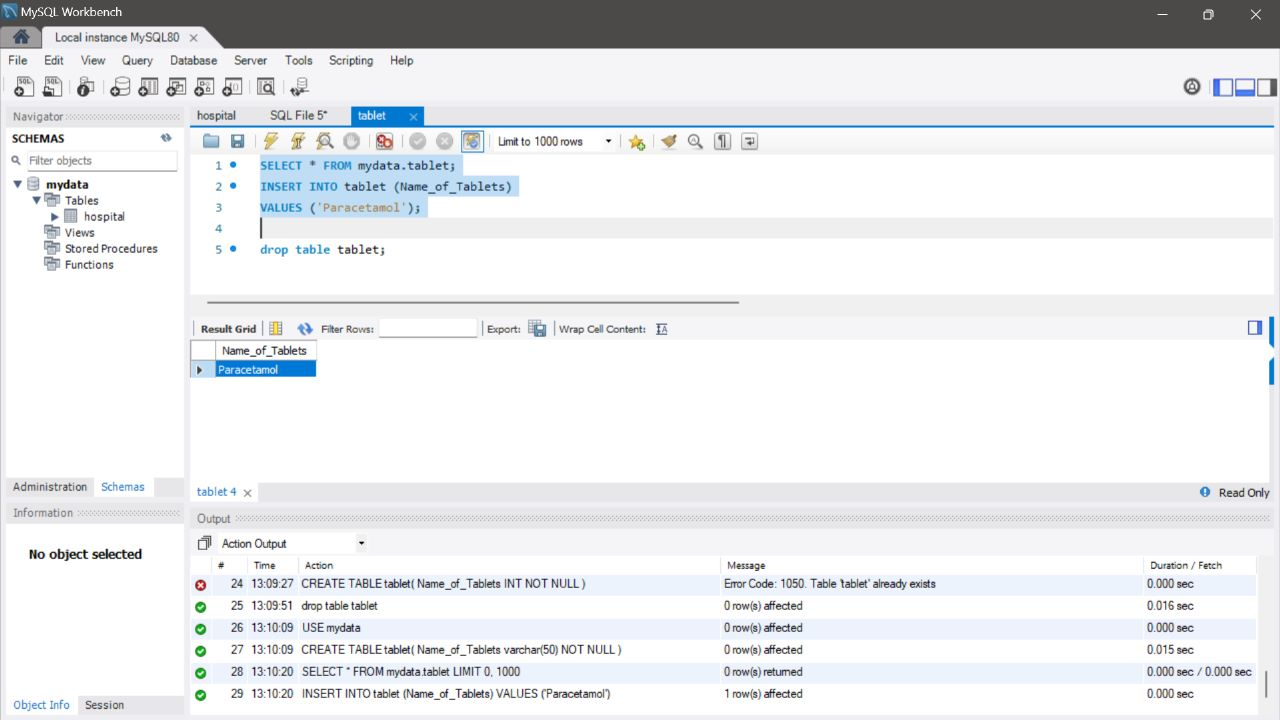
\includegraphics[scale = 0.4]{C1.jpg}
\end{center}

\begin{center}
	\includegraphics*[scale = 0.4]{C2.jpg}
\end{center}

\begin{center}
	\includegraphics*[scale = 0.4]{C3.jpg}
\end{center}

\section{\textbf{Conclusion}}
In conclusion, the hospital management system developed using Python is an efficient and effective solution for managing administrative and clinical workflows in hospitals. The use of Python and Django ensures that the system is scalable, secure, and easy to maintain.

\section{\textbf{Future Scope}}
The hospital management system can be further improved by adding more features, such as electronic medical records, billing and payment systems, and integration with other hospital systems. The system can also be extended to mobile devices, providing real-time access to patient information from anywhere.
\end{document}